\documentclass[BSP,english,oneside]{ntnuthesis/ntnubachelorthesis}

\usepackage{csvsimple}
\usepackage{booktabs}
\usepackage{import} % Used for import from folders.
\usepackage{mathtools}
\usepackage[miktex]{gnuplottex}

\usepackage[T1]{fontenc}
\usepackage[utf8]{inputenc}
\usepackage{lmodern}
\usepackage[miktex]{gnuplottex}
\usepackage{graphicx}
\usepackage{float}
\usepackage[final]{pdfpages}

\usepackage[binary-units=true]{siunitx}
\DeclareSIUnit\year{yr}

\import{../latex_utility/}{listing_cpp_syntax.tex}
\import{../latex_utility/}{pt_commands.tex}

%\renewcommand{\comment}[1]{\textcolor{blue}{\emph{#1}}}  %% use of the colour and you can see how to use commands with parts
\newcommand{\com}[1]{{\color{red}#1}} % supervisor comment
\renewcommand{\com}[1]{} %remove starting % to remove supervisor comments
% This will appear in text \com{Lecuters comment} and be visible unless you uncomment
% the renewcommand line.

\newcommand{\todo}[1]{{\color{cyan}\lbrack todo: #1\rbrack}\\} % items to do
\renewcommand{\todo}[1]{} %remove starting % to remove items to do

\newcommand{\n}[1]{{\color{blue}#1}} % other comment
\renewcommand{\n}[1]{} %remove starting % to remove notes

\newcommand{\dn}[1]{} % add the dn to a note to say that you have finished with it.

% To use when just doing a regular section reference, if more custom wording is needed,
% the footnote must be set up manually
\newcommand{\secref}[1]{\footnote{See section \ref{#1}}}

\newcounter{ptrequirements}
\newcommand{\requirement}[2]{\begin{quote}\refstepcounter{ptrequirements}\textbf{Requirement \theptrequirements: #1 \label{#2}}\end{quote}}
\newcommand{\reqref}[1]{\footnote{Requirement \ref{#1}.}}
\newcommand{\reqcomment}[1]{\emph{Comment: #1}}

\newcommand{\cpp}{\mbox{C++}}
\newcommand{\std}[1]{\mbox{std::#1}}

\def \gnuplotterminal {pdf}
%\newcommand{}{pdf}

\begin{document}

\subimport{inc/}{thesis_data.tex}

\makefrontpages

\subimport{inc/}{preface.tex}
\todo{Haha}

\tableofcontents
\listoffigures
\listoftables
\lstlistoflistings

\subimport{inc/}{introduction.tex}
\subimport{inc/}{requirements.tex}
\subimport{inc/}{technical.tex}
\subimport{inc/}{measurements.tex}
\subimport{inc/}{benchmarking.tex}
\subimport{inc/}{discussion.tex}
\subimport{inc/}{future_work.tex}
\subimport{inc/}{process.tex}
\subimport{inc/}{conclusion.tex}

\bibliographystyle{ntnuthesis/ntnubachelorthesis}
\bibliography{inc/thesis}



\appendix %after this line all chapters will have leters instead of numbers
\chapter{Massif Memory Output}
\label{chap:appendix_massif_output}
\begin{figure}
    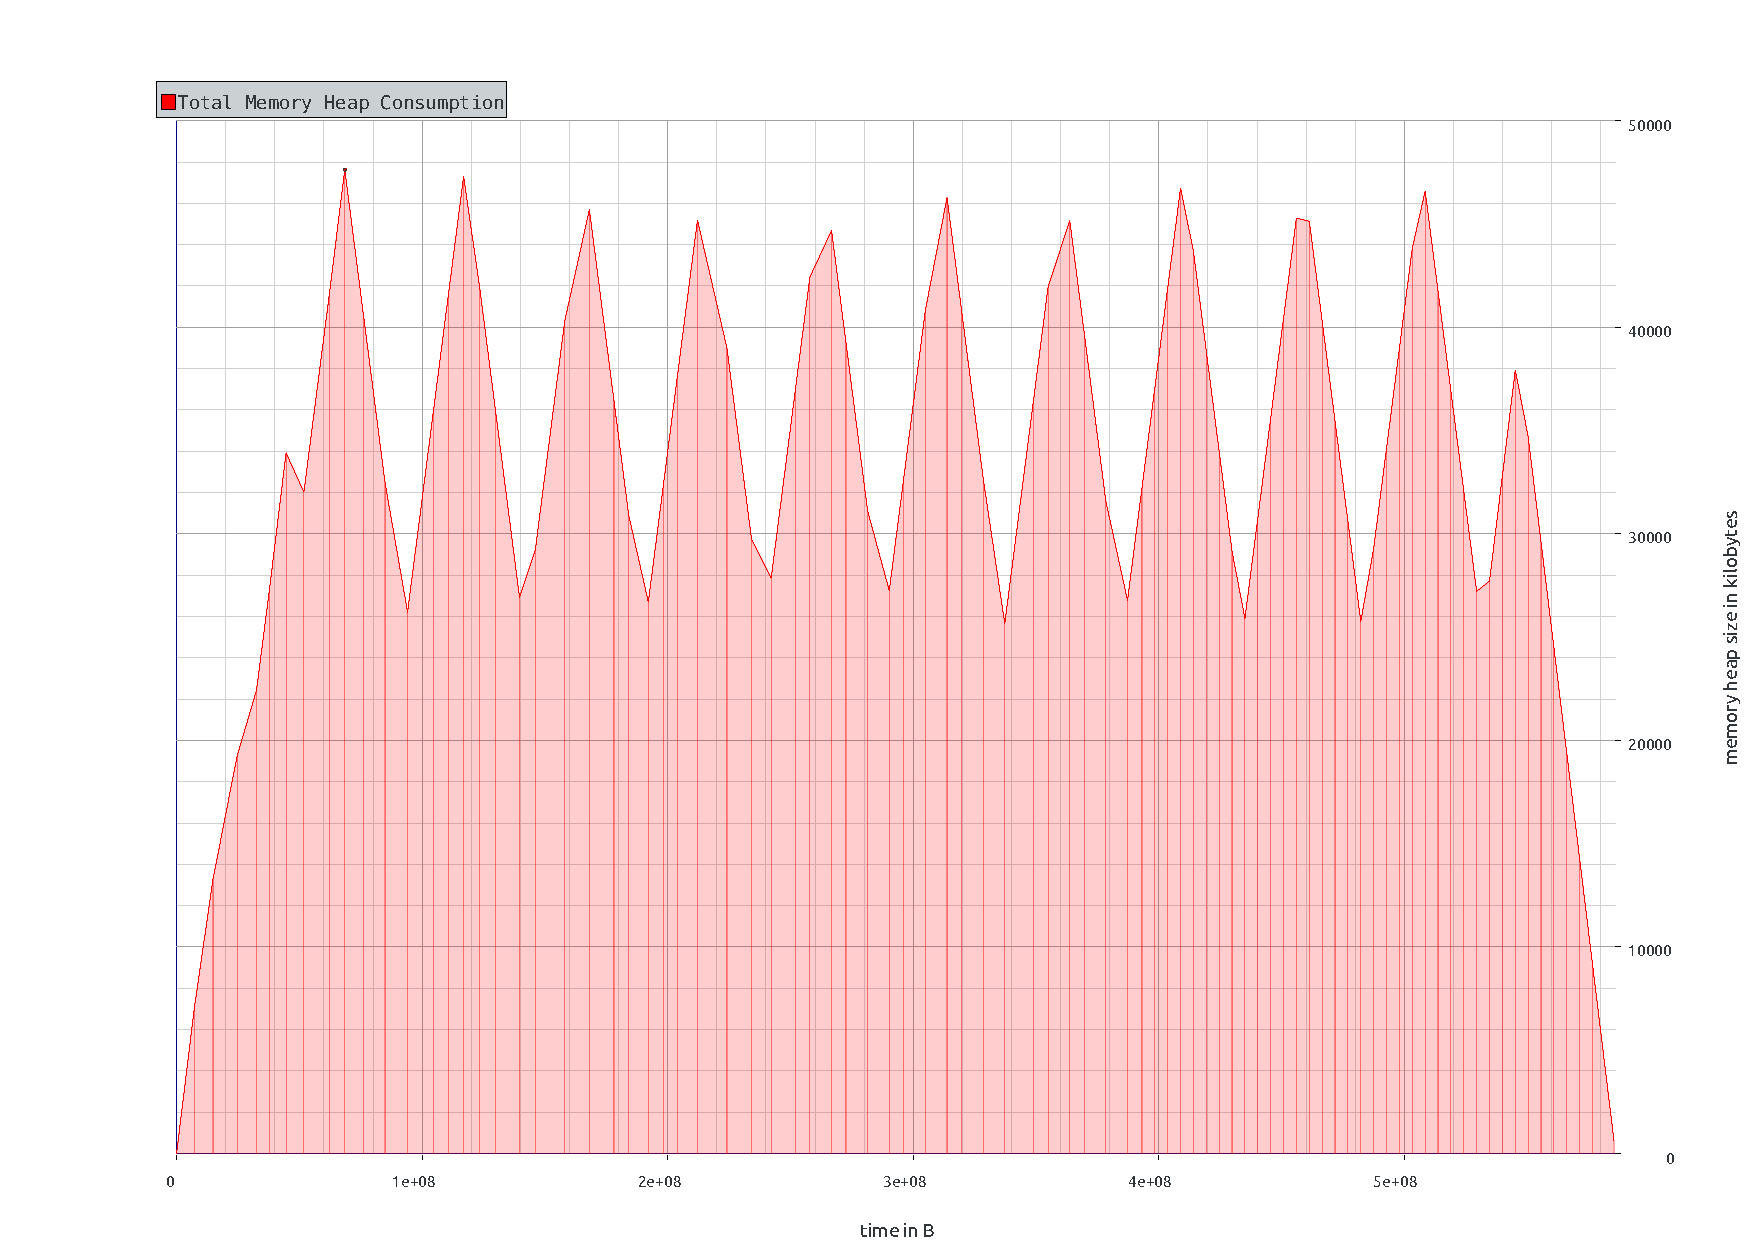
\includegraphics[scale=0.5]{benchmark_results/fast_spawn/ecs_massif_deletes_10.pdf}
    \caption{Fast spawning memory usage, NOX ECS}
\end{figure}

\begin{figure}
    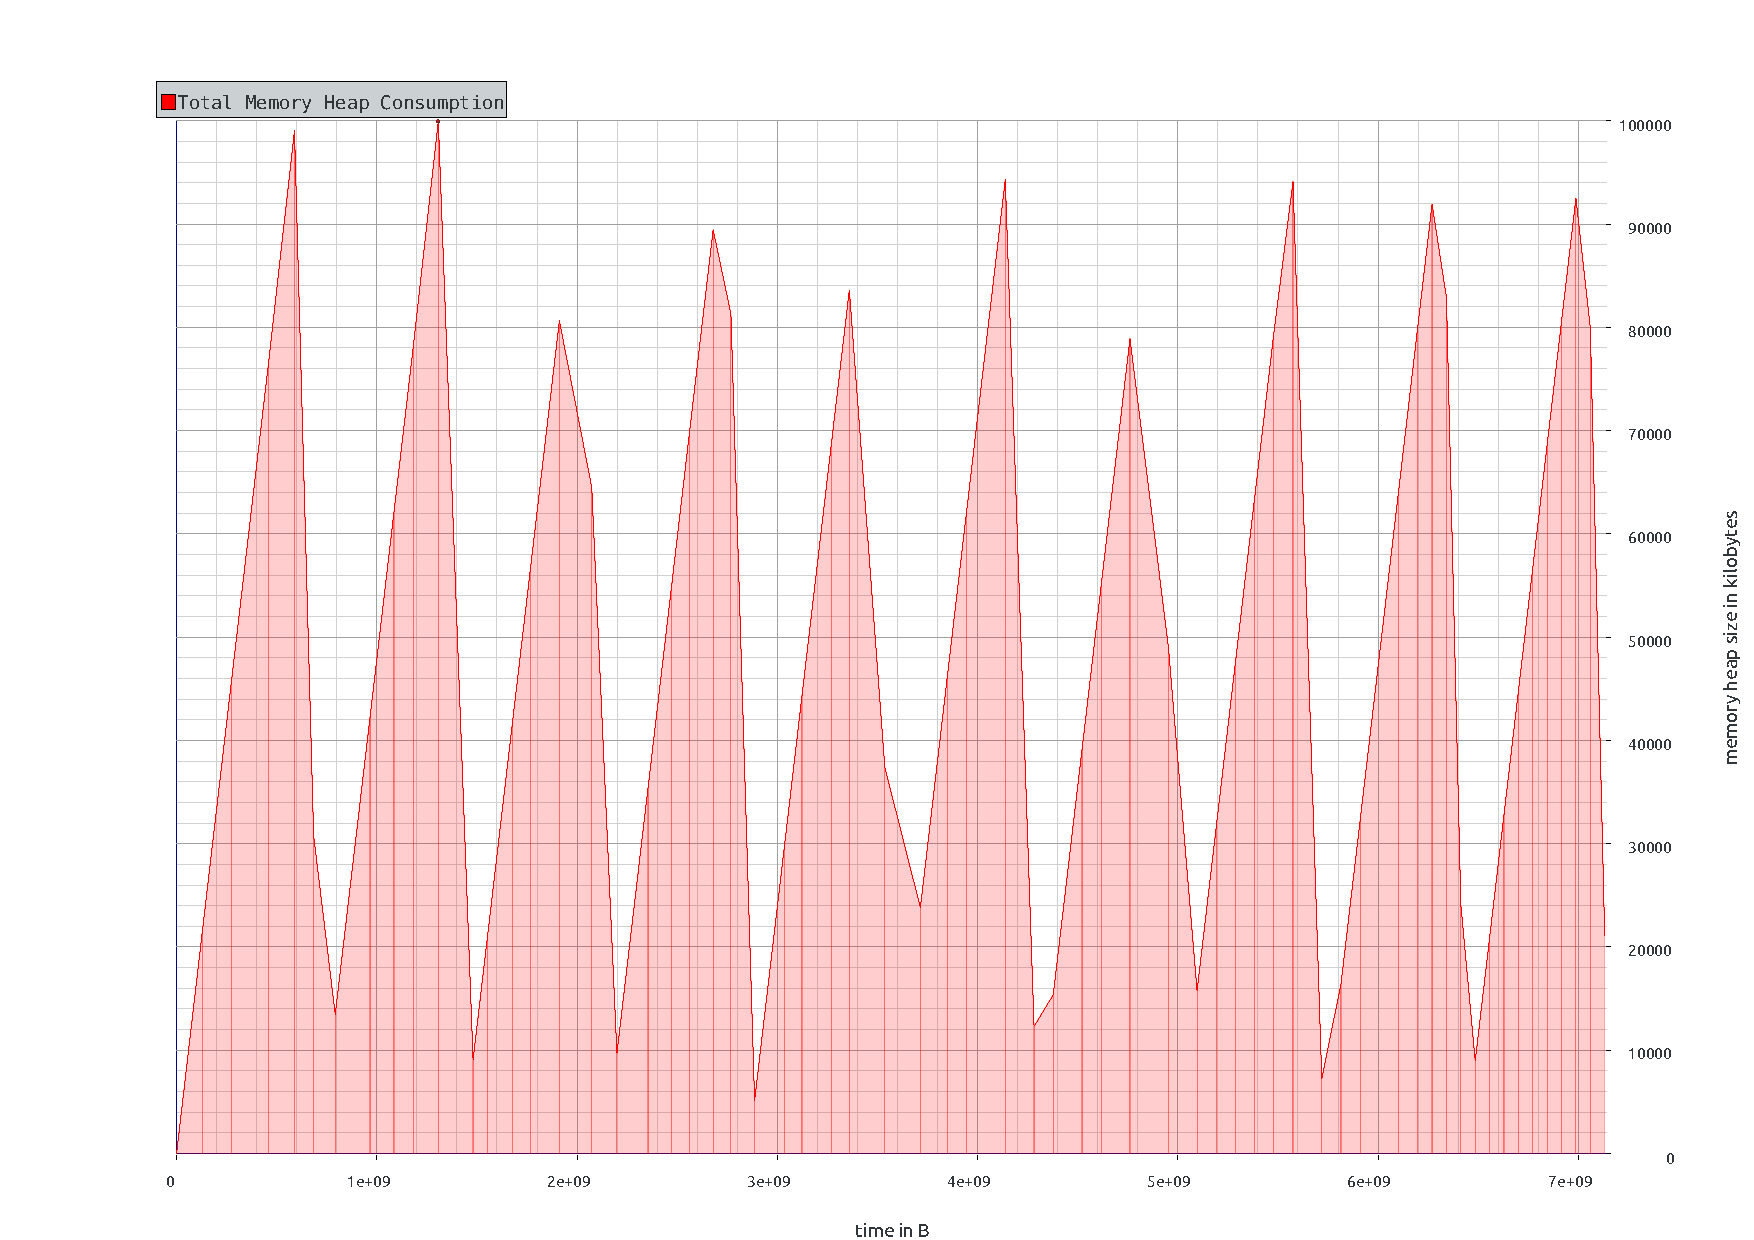
\includegraphics[scale=0.5]{benchmark_results/fast_spawn/nox_massif_deletes_10.pdf}
    \caption{Fast spawning memory usage, NOX Actor}
\end{figure}

\chapter{Hardware Info}
\label{chap:hardware_info}
\subimport{inc/}{hardware_info.tex}

\chapter{Code}
\label{chap:code}
\subimport{inc/}{code.tex}

\chapter{Data}
\label{chap:data}
The various data recorded from the tests can be found in the results folder on the development repository.

\chapter{Test Case Plan}
\label{chap:appendix_test_case_plan}
The following appendix includes the test case plan, which the tests were based upon.

\includepdf[pages=-]{../test_case_plan/build/test_case_plan_format.pdf}

\chapter{Technical Specification}
\label{chap:appendix_technical_specification}
The technical specification outlines addition requirements on the functionality of the NOX ECS.
\includepdf[pages=-]{../technical_specification/build/technical_specification.pdf}

\chapter{Design Document}
\label{chap:appendix_design_document}
The Design document was created when prototyping NOX ECS, and shows the original ideas of the system.
\includepdf[pages=-]{../design_document/build/design_document.pdf}

\chapter{Project Plan}
\label{chap:appendix_project_plan}
The project plan shows our original plan for the project and topic. Both the topic and the plan changed
quite a bit during development.

\includepdf[pages=-]{../project_plan/compiled_pdf/o7_project_plan.pdf}

\chapter{Scrum Plan v2}
\label{chap:appendix_scrum_plan_v2}
The scrum plan v2, contains the new sprints after the first re-planning process.
\includepdf[pages=-]{../scrum_plan_v2/build/scrum_plan_v2.pdf}

\chapter{Scrum Plan v3}
\label{chap:appendix_scrum_plan_v3}
The scrum plan v3, containes the new sprints after the second re-planning process.
\includepdf[pages=-]{../scrum_plan_v3/build/scrum_plan_v3.pdf}

\chapter{Sprint Retrospectives}
\label{chap:appendix_sprint_retrospectives}
This appendix includes the different sprint retrospectives that were held during the development.
\includepdf[pages=-]{../sprint_retrospectives/build/280217.pdf}
\includepdf[pages=-]{../sprint_retrospectives/build/080317.pdf}
\includepdf[pages=-]{../sprint_retrospectives/build/190317.pdf}
\includepdf[pages=-]{../sprint_retrospectives/build/280317.pdf}
\includepdf[pages=-]{../sprint_retrospectives/build/030417.pdf}

\chapter{Stakeholder Meetings}
\label{chap:appendix_stakeholder_meetings}
Following are the summaries from the different meetings with the stakeholder.
\includepdf[pages=-]{../stakeholder_meetings/build/060217.pdf}
\includepdf[pages=-]{../stakeholder_meetings/build/210217.pdf}
\includepdf[pages=-]{../stakeholder_meetings/build/220317.pdf}
\includepdf[pages=-]{../stakeholder_meetings/build/280217.pdf}

\chapter{Supervisor Meetings}
\label{chap:appendix_supervisor_meetings}
Following are the summaries from the different meetings with the supervisor.
\includepdf[pages=-]{../supervisor_meetings/build/100217.pdf}
\includepdf[pages=-]{../supervisor_meetings/build/160217.pdf}
\includepdf[pages=-]{../supervisor_meetings/build/080317.pdf}
\includepdf[pages=-]{../supervisor_meetings/build/240317.pdf}

\chapter{Daily Scrum Meetings}
\label{chap:appendix_daily_scrum_meetings}
\includepdf[pages=-]{../daily_scrum/build/010217.pdf}
\includepdf[pages=-]{../daily_scrum/build/020217.pdf}
\includepdf[pages=-]{../daily_scrum/build/030217.pdf}
\includepdf[pages=-]{../daily_scrum/build/060217.pdf}
\includepdf[pages=-]{../daily_scrum/build/070217.pdf}
\includepdf[pages=-]{../daily_scrum/build/080217.pdf}
\includepdf[pages=-]{../daily_scrum/build/100217.pdf}
\includepdf[pages=-]{../daily_scrum/build/130217.pdf}
\includepdf[pages=-]{../daily_scrum/build/140217.pdf}
\includepdf[pages=-]{../daily_scrum/build/150217.pdf}
\includepdf[pages=-]{../daily_scrum/build/200217.pdf}
\includepdf[pages=-]{../daily_scrum/build/210217.pdf}
\includepdf[pages=-]{../daily_scrum/build/220217.pdf}
\includepdf[pages=-]{../daily_scrum/build/250217.pdf}
\includepdf[pages=-]{../daily_scrum/build/260217.pdf}
\includepdf[pages=-]{../daily_scrum/build/280217.pdf}
\includepdf[pages=-]{../daily_scrum/build/010317.pdf}
\includepdf[pages=-]{../daily_scrum/build/060317.pdf}
\includepdf[pages=-]{../daily_scrum/build/070317.pdf}
\includepdf[pages=-]{../daily_scrum/build/080317.pdf}
\includepdf[pages=-]{../daily_scrum/build/100317.pdf}
\includepdf[pages=-]{../daily_scrum/build/110317.pdf}
\includepdf[pages=-]{../daily_scrum/build/200317.pdf}
\includepdf[pages=-]{../daily_scrum/build/210317.pdf}
\includepdf[pages=-]{../daily_scrum/build/220317.pdf}
\includepdf[pages=-]{../daily_scrum/build/240317.pdf}
\includepdf[pages=-]{../daily_scrum/build/250317.pdf}
\includepdf[pages=-]{../daily_scrum/build/260317.pdf}
\includepdf[pages=-]{../daily_scrum/build/270317.pdf}
\includepdf[pages=-]{../daily_scrum/build/280317.pdf}
\includepdf[pages=-]{../daily_scrum/build/290317.pdf}
\includepdf[pages=-]{../daily_scrum/build/310317.pdf}
\includepdf[pages=-]{../daily_scrum/build/020417.pdf}
\includepdf[pages=-]{../daily_scrum/build/030417.pdf}
\includepdf[pages=-]{../daily_scrum/build/040417.pdf}
\includepdf[pages=-]{../daily_scrum/build/050417.pdf}
\includepdf[pages=-]{../daily_scrum/build/210417.pdf}
\includepdf[pages=-]{../daily_scrum/build/220417.pdf}
\includepdf[pages=-]{../daily_scrum/build/230417.pdf}
\includepdf[pages=-]{../daily_scrum/build/240417.pdf}
\includepdf[pages=-]{../daily_scrum/build/250417.pdf}
\includepdf[pages=-]{../daily_scrum/build/300417.pdf}
\includepdf[pages=-]{../daily_scrum/build/010517.pdf}
\includepdf[pages=-]{../daily_scrum/build/020517.pdf}
\includepdf[pages=-]{../daily_scrum/build/040517.pdf}
\includepdf[pages=-]{../daily_scrum/build/050517.pdf}
\includepdf[pages=-]{../daily_scrum/build/060517.pdf}
\includepdf[pages=-]{../daily_scrum/build/070517.pdf}
\includepdf[pages=-]{../daily_scrum/build/090517.pdf}
\includepdf[pages=-]{../daily_scrum/build/100517.pdf}
\includepdf[pages=-]{../daily_scrum/build/110517.pdf}
\includepdf[pages=-]{../daily_scrum/build/120517.pdf}



%\chapter{Scrum Plans}
%\chapter{Daily Scrum Logs}
%\chapter{Stakeholder Meetings}
%\chapter{Supervisor Meetings}
%\chapter{Sprint Retrospectives}
%\chapter{Group Rules}
%\chapter{Benchmark Data}
%\chapter{Stakeholder Contract}




%Give short explanation on how to see the cachegrind stuff.
%
\end{document}
